%
% =============================================================================
%
%                                   Premable
%
% =============================================================================
%

\documentclass{book}
\usepackage{fullpage}
\usepackage{pylal}


% Add your name to the author list!  (alphabetical order?)

\title{pyLAL Applications User Guide and Reference}
\author{Kipp Cannon, Thomas Cokelaer, Alexander Dietz, Steve Fairhurst}
\date{\today}


%
% =============================================================================
%
%                                   Document
%
% =============================================================================
%

\begin{document}
\maketitle
\tableofcontents
\listoftables
\listoffigures
\chapter{Coding Conventions}
\section{General}
The executables should contain some standard code at the beginning of the
document such as
%
\begin{verbatim}
__author__ = "Albert Einstein <albert.einstein@ligo.org>
\end{verbatim}
to identify the author. If you parse arguments with the \prog{optparse}
module, be sure to do \progarg{from pylal import git\_version} and in the
parser initialization, use the kwarg
\progarg{version=git\_version.verbose\_msg} in order to support
\progarg{--version}.

\section{Naming conventions}
The output file should be 
\begin{verbatim}
<executable name>_<usertag>_<figure name>-<GPS start time>-<duration>.png
<executable name>_<usertag>-<GPS start time>-<duration>.html
<executable name>_<usertag>-<GPS start time>-<duration>.cache
\end{verbatim}
Where, executable name is defined by the variable \prog{\_\_name\_\_} (see above)


\section{Optional arguments}
The are numerous options available in the pylal plotting functions. Some of
them should be standarize. In particular, we identify the following options,
which should be present in the list of avaialable options :

\begin{description}
\item[\progarg{--output-cache}] to be used to provide a cache file
\item[\progarg{--output-html}] to be used to provide a cache file
\item[\progarg{--output-path}] to be used to provide a cache file
\item[\progarg{--gps-start-time}] to be used to provide a cache file
\item[\progarg{--gps-end-time}] to be used to provide a cache file
\item[\progarg{--figure-name}] a tag to be used for naming the output figures
(see Naming conventions).
\item[\progarg{--verbose}] Be verbose
\end{description}

There are others option, which could be standarize such as the one related to
globing or input cache file.


\section{TODO}
sort the list of arguments by alphabetical order.



\chapter{Burst Tools}
\begin{manpage}{\prog{ligolw\_binjfind}}

\manname{\prog{ligolw\_binjfind}}{A program for finding burst injections.}

\mansynopsis{\prog{ligolw\_binjfind} \{\progarg{-c},\progarg{--match-algorithm}\} \progparm{algorithm} [options] [file [file ...]]}

\begin{mansection}{Description}
\prog{ligolw\_binjfind} applies a burst injection identification algorithm
to one or more LIGO Light Weight XML files, each containing a list of burst
triggers and a list of software injections.  If no file names are provided
on the command line, then input is read from \file{stdin}, and output
written to \file{stdout}.  Any file whose name ends in ``\file{.gz}'' is
assumed to be gzip-compressed.

The results of the search are recorded using the standard coincidence table
infrastructure.
\end{mansection}

\begin{mansection}{Options}
\begin{description}
\item[\progarg{--comment} \progparm{text}] Set the string to be recorded as
the comment in the job metadata added to the files.  The default is ``''.

\item[\progarg{-f},\progarg{--force}] Normally input files whose internal
metadata indicates they have already been processed will be skipped.  This
behaviour facilitates the use of \prog{ligolw\_binjfind} in Condor DAGs,
where it is convenient to have one job process many files but where a job
may be evicted and re-started, causing it to re-read each file.  Setting
\progarg{--force} forces files to be re-processed.

\item[\progarg{-h},\progarg{--help}] Show a help message and exit.

\item[\progarg{-c},\progarg{--match-algorithm} \progparm{algorithm}] Set
the algorithm to be used in comparing burst triggers to injections.  There
are currently two algorithms defined, \progarg{excesspower} and
\progarg{stringcusp}.  The former is suitable for use in comparing the
triggers generated by \prog{lalapps\_power} to a list of burst injections,
while the latter is for use in comparing the triggers generated by
\prog{lalapps\_StringSearch}.

\item[\progarg{--verbose}] Be verbose.

\item[\progarg{--version}] Show program's version number and exit.

\end{description}
\end{mansection}

\begin{mansection}{See Also}
\prog{ligolw\_add}, \prog{lalapps\_binj}, \prog{ligolw\_burca}
\end{mansection}

\end{manpage}

\chapter{Inspiral Tools}
\begin{manpage}{\prog{plotnumtemplates}}

\manname{\prog{plotnumtemplates}}{A program for plotting template bank size.}
\mansynopsis{\prog{plotnumtemplates}  [options] }

\begin{mansection}{Description}
\prog{plotnumtemplates} scan template and/or triggered template bank, 
search for nevents in the summary table and create a pictures combining 
the template bank sizes for each ifo provided.  Any file whose name ends
in ``\file{.gz}'' is assumed to be gzip-compressed.

The results of the search can be stored in a png figure.
\end{mansection}

\begin{mansection}{Options}
\begin{description}
\item[to be done]

\item[\progarg{--verbose}] Be verbose.

\item[\progarg{--version}] Show program's version number and exit.

\end{description}
\end{mansection}

\begin{mansection}{See Also}
\prog{plotnumtriggers}, \prog{plotinspiral}
\end{mansection}

\end{manpage}

\begin{manpage}{\prog{plotinspiralrange}}

\manname{\prog{plotinspiralrange}}{A program for plotting inspiral horizon distance.}
\mansynopsis{\prog{plotinspiralrange}  [options] }

\begin{mansection}{Description}
\prog{plotinspiralrange} scan template bank files, 
search for horizon distance in summary table 
and create 3  pictures of horizon distance for a standard BNS first, and for
the mass range provided.  Any file whose name ends
in ``\file{.gz}'' is assumed to be gzip-compressed.

The results of the search are  stored in a png format.
\end{mansection}


\begin{mansection}{Options}
\begin{description}
\item[\progarg{--version}] show program's version number and exit
\item[\progarg{-h, --help}] show this help message and
\item[\progarg{-I INSP, --inspiral-glob=INSP}]     glob for files containing the string INSP
\item[\progarg{-c CACHE, --cache-file=CACHE}]    name of cache file with details if
\item[\progarg{-s, --show-plot}] display the figures on the
\item[\progarg{-m MIN, --range-min=MIN}]     minimum value on range plots  
\item[\progarg{-M MAX, --range-max=MAX}]     maximum value on range plots  
\item[\progarg{-a, --range-vs-time}]  make a plot of range
\item[\progarg{-b, --range-hist}]  make a histogram of the
\item[\progarg{--range-mass}]  make a plot of the range
\item[\progarg{--mass-min=MIN}]  minimum x-value on mass plots 
\item[\progarg{--mass-max=MAX}]  maximum x-value on mass plots 
\item[\progarg{-t PLOT\_TYPE, --plot-type= PLOT\_TYPE}]    make either linear or log or plots
\item[\progarg{-n NBINS, --nbins=NBINS }]    number of bins for range hist (default
\item[\progarg{-f FNAME, --figure-name= FNAME}]   generate png figures with name FNAME-fig.png 
\item[\progarg{-W, --output-html}] generate a html page containing
\item[\progarg{-C, --output-cache}] generate a cache file with
\item[\progarg{-P PATH, --output-path=PATH}]     path where the figures would be stored
\item[\progarg{-S GPSSTART, --gps-start-time=GPSSTART}]    gps start time (for naming figure and
\item[\progarg{-E GPSEND, --gps-end-time= GPSEND}]   gps end time (for naming figure and
\item[\progarg{-v, --verbose}] print information   
\end{description}
\end{mansection}


\begin{mansection}{Output}
This program returns three png images such in
figure\ref{fig:lalapps_plotinspiralrange}, an html file and a cache file (if
ouptut-html and output-cache are provided). The output filenames follow the
naming convention : 

plotinspiralrange\_usertag\_figurename-gpsstart-duration


\begin{figure}[ht]
{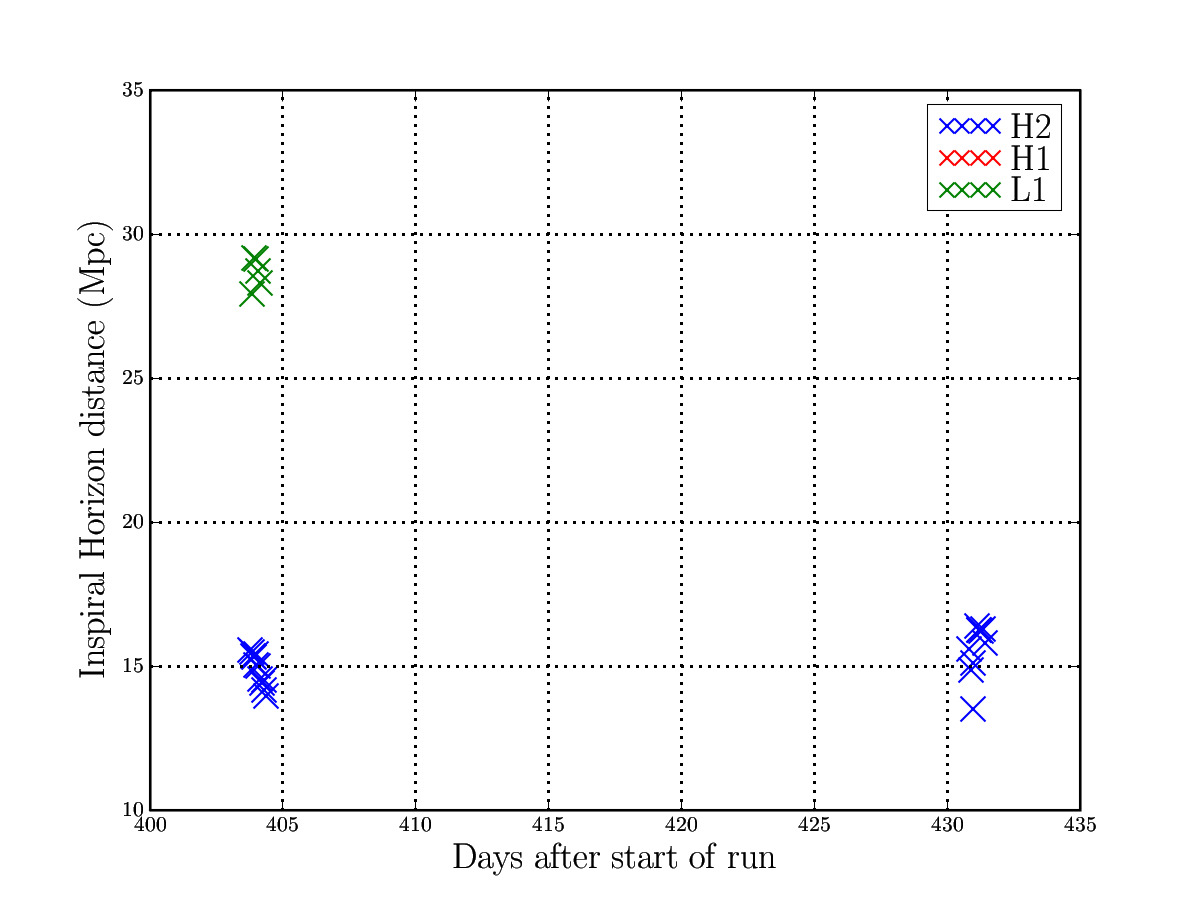
\includegraphics[width=0.30\textwidth]{./plotinspiralrange_playground_range_plot-849974770-2419200.png}}
{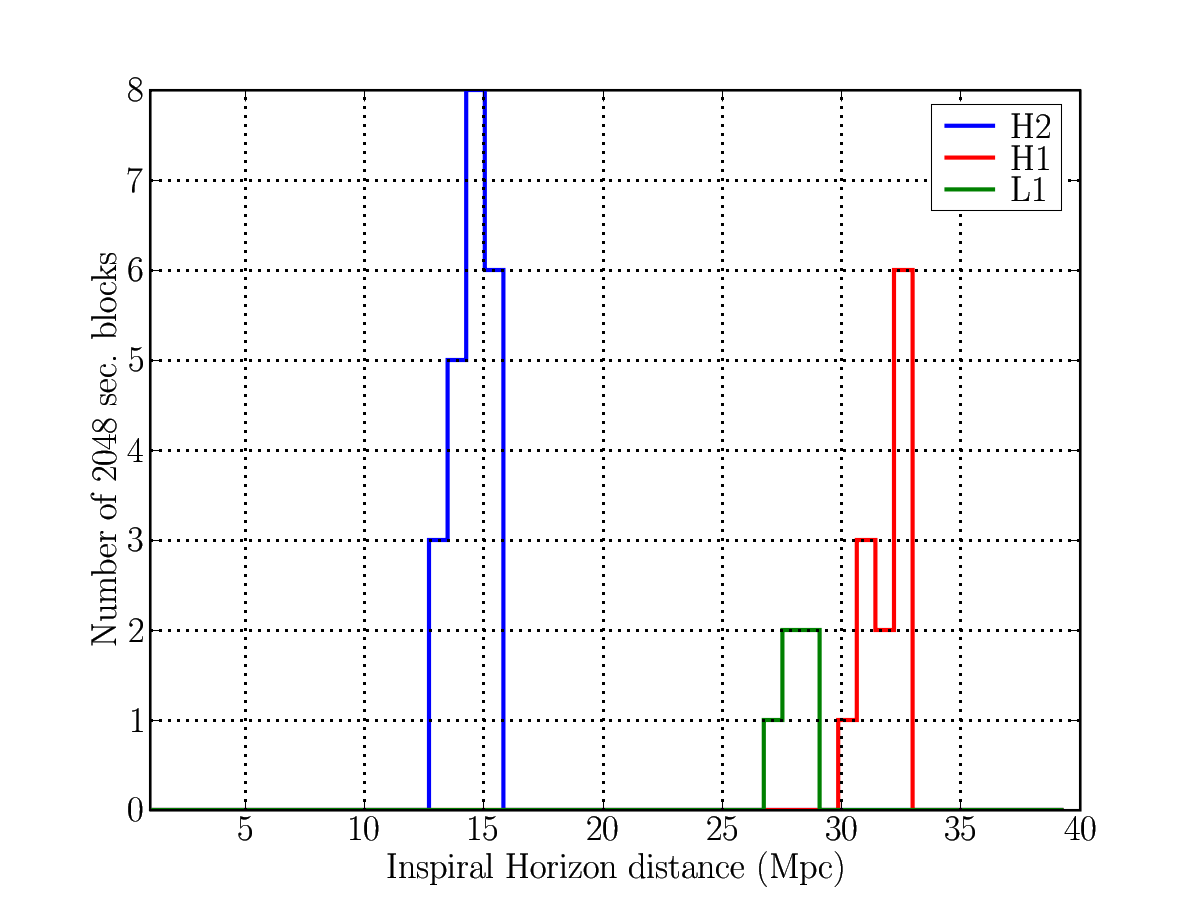
\includegraphics[width=0.30\textwidth]{./plotinspiralrange_playground_range_hist-849974770-2419200.png}}
{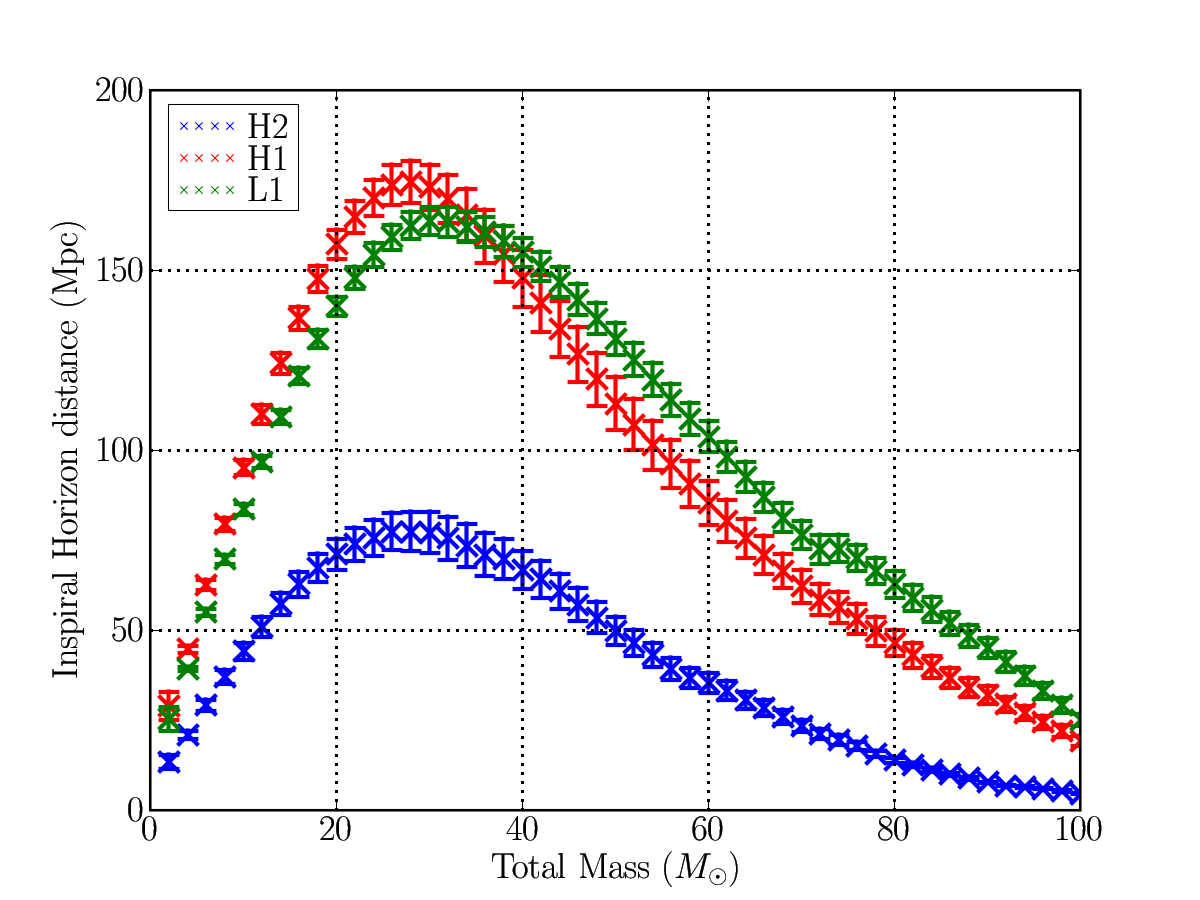
\includegraphics[width=0.30\textwidth]{./plotinspiralrange_playground_range_mass-849974770-2419200.png}}
\caption{\label{fig:lalapps_plotinspiralrange} test}
\end{figure}
\end{mansection}

\begin{mansection}{Examples}
\begin{verbatim}
~/opt/pylal/bin/lalapps_plotinspiralrange --cache-file  test.cache   -f
playground --range-min 1 --range-max 40 --n 50 --range-vs-time --range-hist
--verbose -a -b --range-mass --gps-start-time 849974770 --gps-end-time
852393970  --output-cache --output-html --output-path playground --help
\end{verbatim}
\end{mansection}



\begin{mansection}{See Also}
\prog{plotnumtriggers}, \prog{plotinspiral}
\end{mansection}

\end{manpage}

\clearpage


\end{document}
